\let\negmedspace\undefined
\let\negthickspace\undefined
\documentclass[journal]{IEEEtran}
\usepackage[a5paper, margin=10mm, onecolumn]{geometry}
%\usepackage{lmodern} % Ensure lmodern is loaded for pdflatex
\usepackage{tfrupee} % Include tfrupee package

\setlength{\headheight}{1cm} % Set the height of the header box
\setlength{\headsep}{0mm}     % Set the distance between the header box and the top of the text

\usepackage{gvv-book}
\usepackage{gvv}
\usepackage{cite}
\usepackage{amsmath,amssymb,amsfonts,amsthm}
\usepackage{algorithmic}
\usepackage{graphicx}
\usepackage{textcomp}
\usepackage{xcolor}
\usepackage{txfonts}
\usepackage{listings}
\usepackage{enumitem}
\usepackage{mathtools}
\usepackage{gensymb}
\usepackage{comment}
\usepackage[breaklinks=true]{hyperref}
\usepackage{tkz-euclide} 
\usepackage{listings}
% \usepackage{gvv}                                        
\def\inputGnumericTable{}                                 
\usepackage[latin1]{inputenc}                                
\usepackage{color}                                            
\usepackage{array}                                            
\usepackage{longtable}                                       
\usepackage{calc}                                             
\usepackage{multirow}                                         
\usepackage{hhline}                                           
\usepackage{ifthen}                                           
\usepackage{lscape}
\begin{document}

\bibliographystyle{IEEEtran}
\vspace{3cm}

\title{9.5.11}
\author{EE25BTECH11049 - Sai Krishna Bakki}
\maketitle
\textbf{Question:}\\
Two pipes running together can fill a tank in 100/9 minutes. If one pipe takes 5 minutes more than the other to fill the tank separately, find the time in which each pipe would
fill the tank separately.

\solution\\
Given:\\
Let the time taken by the faster pipe to fill the tank be \textbf{'x'} minutes and the time taken by the slower pipe to fill the tank be \textbf{'x+5'} minutes.\\
The amount of the tank each pipe fills in one minute is its work rate.
\begin{itemize}
    \item Work rate of the first pipe = $\frac{1}{x}$
    \item Work rate of the second pipe = $\frac{1}{x+5}$
\end{itemize}
When working together, they fill the tank in $\frac{100}{9}$ minutes. Therefore, their combined work rate is the reciprocal,$\frac{9}{100}$ of the tank per minute.
\begin{align}
    \frac{1}{x}+\frac{1}{x+5}=\frac{9}{100}\\
    \frac{2x+5}{x^2+5x}=\frac{9}{100}\\
    \implies y=9x^2-155x-500=0\label{eq:conic}
\end{align}
which can be expressed as the conic
\begin{align}
\vec{x}^{T}\vec{V}\vec{x}+2\vec{u}^T\vec{x}+f=0\\
\vec{V}=\myvec{9&0\\0&0},\vec{u}=\myvec{\frac{-155}{2}\\\frac{-1}{2}},f=-500
\end{align}
To find the roots of $\eqref{eq:conic}$, we find the points of intersection of the conic with the x-axis
\begin{align}
    \vec{x}=\vec{h}+\kappa\vec{m}\\
    \vec{h}=\myvec{0\\0},\vec{m=\myvec{1\\0}}
\end{align}
The parameter $\kappa$ for the points of intersection is found using the formula:
\begin{align}
\kappa = \frac{1}{\vec{m}^\top \vec{V} \vec{m}}\brak{-\vec{m}^\top(\vec{V}\vec{h}+\vec{u}) \pm \sqrt{\sbrak{\vec{m}^\top(\vec{V}\vec{h}+\vec{u})}^2 - g(\vec{h})(\vec{m}^\top \vec{V} \vec{m})}}\label{eq:formula}
\end{align}
where $g(\vec{h}) = \vec{h}^\top \vec{V} \vec{h} + 2\vec{u}^\top \vec{h} + f$.\\
using $\eqref{eq:formula}$. The values of $\kappa$ are given by
\begin{align}
    \kappa_i=\frac{1}{9}\brak{\frac{155}{2}\pm\sqrt{\brak{\frac{-155}{2}}^{2}+4500}}\\
    \implies \kappa_1=20,\kappa_2=\frac{-25}{9}
\end{align}
Hence the points of intersection are
\begin{align}
    \vec{h}+\kappa\vec{m}=\myvec{20\\0}\myvec{\frac{-25}{9}\\0}
\end{align}
Hence the solutions of \eqref{eq:conic} are x=20 and x=$\frac{-25}{9}$.
    \begin{figure}[H]
    \centering
    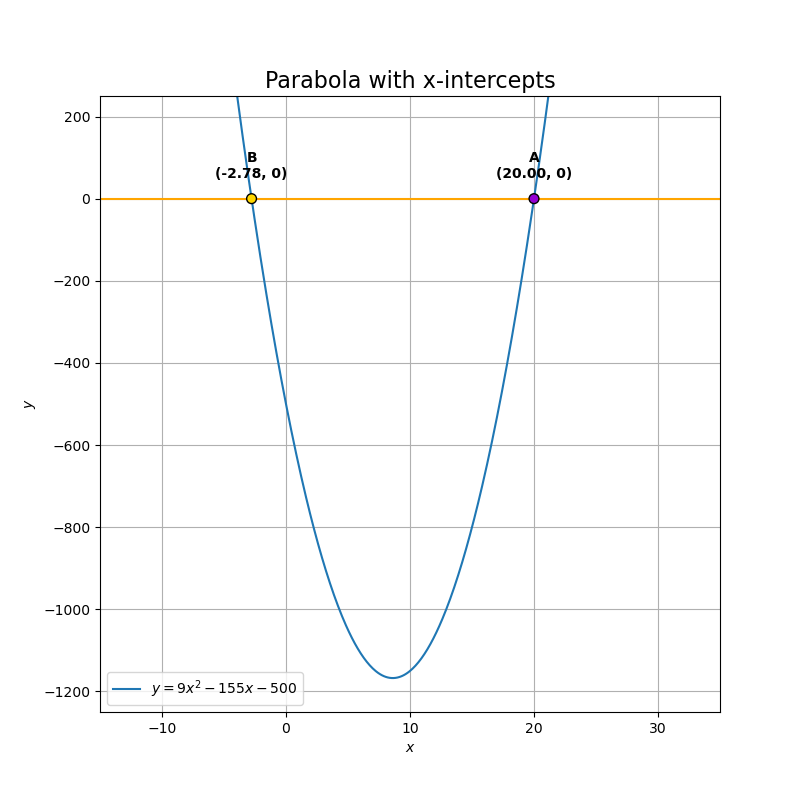
\includegraphics[width=0.7\columnwidth]{figs/Figure_1.png}
    \label{fig:placeholder}
    \caption{}
\end{figure}
\end{document}
